\section{Une lampe dévissée}

Marine a réalisé un circuit ; elle a fait le montage suivant :

\begin{center}
	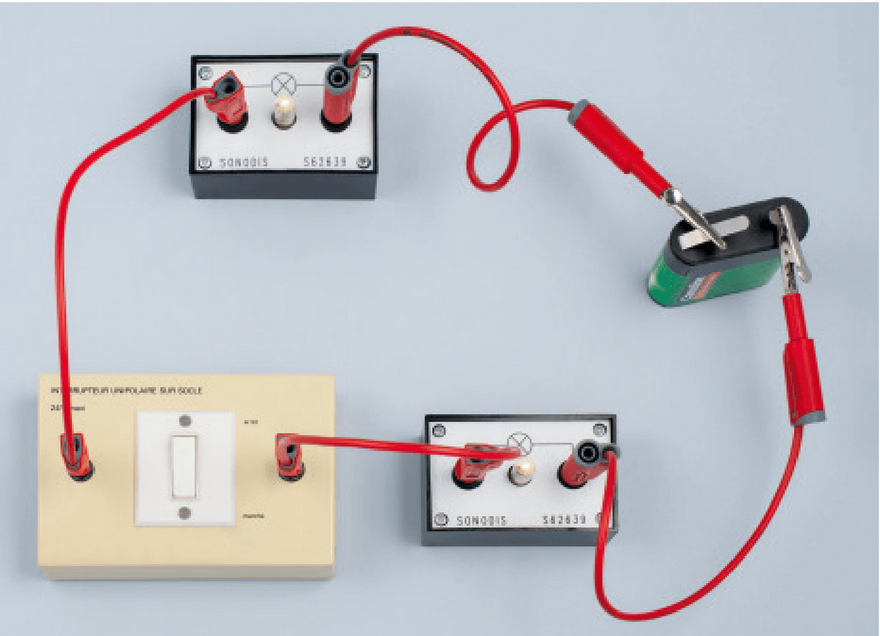
\includegraphics[scale=0.3]{img/circuit_A}
\end{center}

\begin{questions}
	\question Expliquer de quel type de montage il s'agit.
	
	\question Schématiser le circuit.
	
	\question Que se passe-t-il si on dévisse une lampe ?
	
\begin{center}
	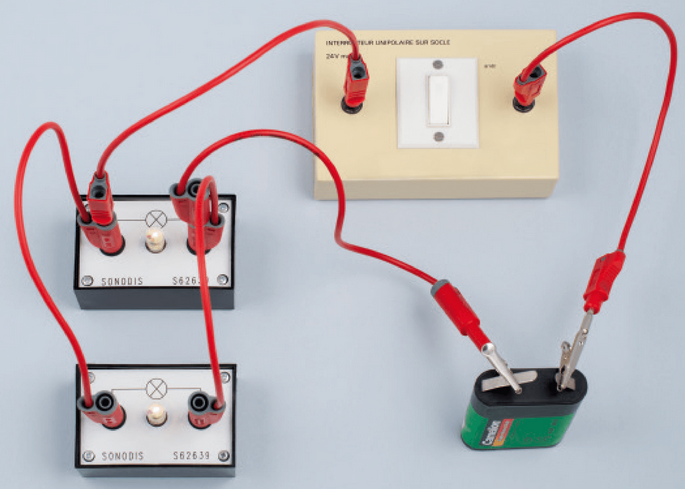
\includegraphics[scale=0.35]{img/circuit_B}
\end{center}
	Avec le même matériel et quelques fils en plus, Clément a réalisé un autre circuit.
	
	\question Expliquer de quel type de montage il s'agit.
	
	\question Schématiser le circuit.
	
	\question Que se passe-t-il si on dévisse une lampe ? Détailler la réponse en utilisant la notion de boucle de courant.
	
	\question Quel type de montage est utilisé pour réaliser les installations électriques des maisons et pourquoi ?
		
\end{questions}
